\documentclass[a4paper,12pt]{article}
\usepackage[utf8]{inputenc}
\usepackage{graphicx}
\usepackage{tcolorbox}
\usepackage{geometry}
\usepackage{setspace} 
\usepackage[absolute,overlay]{textpos} % 引入 textpos 包
\geometry{left=0.8in, right=0.8in, top=1in, bottom=1in}

\begin{document}
	
	\begin{center}
		\Large \textbf{The People's Republic of China \\ Resident Identification Card Translation}
	\end{center}
	
	\vspace{1cm}
	
	% 左右布局
	\noindent
	\begin{minipage}[t]{0.47\textwidth}
		% 人像面
		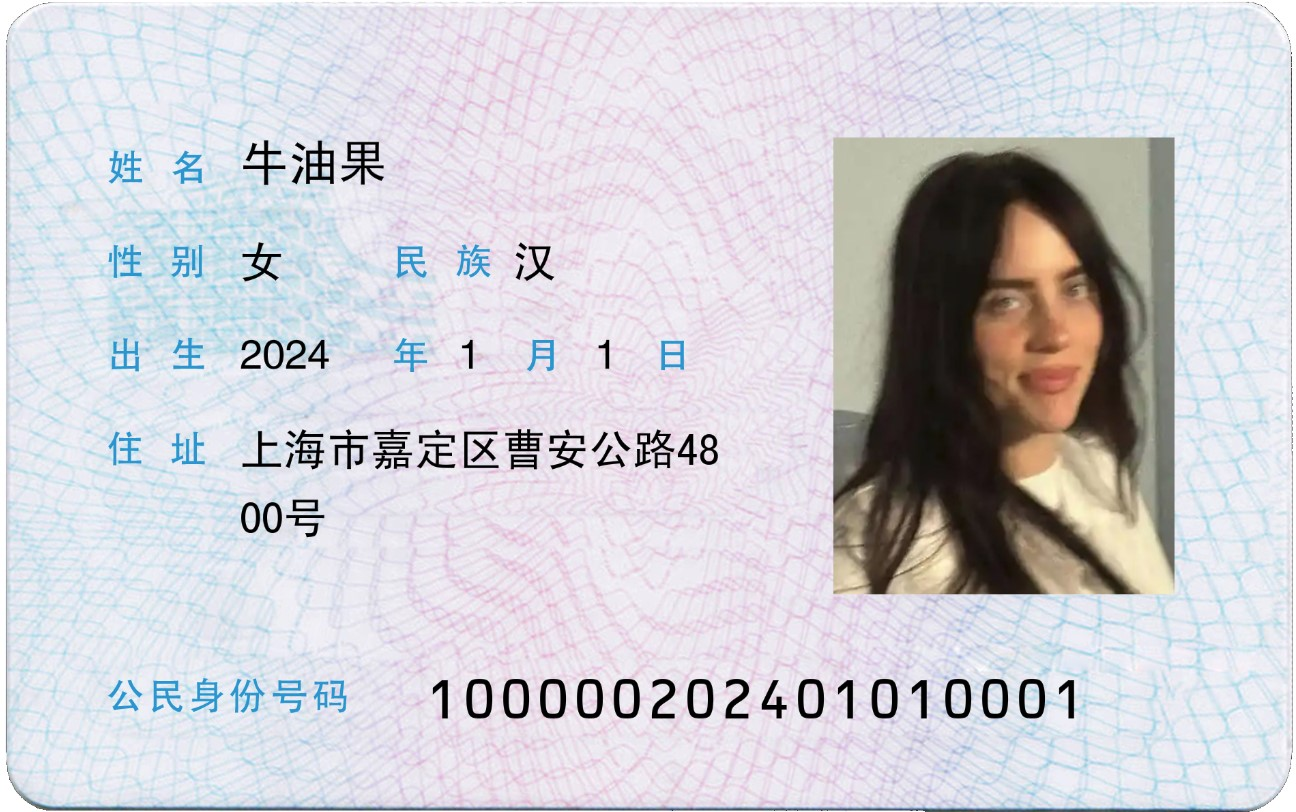
\includegraphics[width=\textwidth]{image/front.jpg} 
	\end{minipage}%
	\hfill
	\begin{minipage}[t]{0.51\textwidth}
		\begin{textblock*}{2cm}(16.5cm,6cm) % 可以自行增加个人照片:设置图片的位置,(x, y) 为起始坐标
			%\includegraphics[width=2cm]{image/profile.jpg} 
		\end{textblock*}
		% translation
		\begin{tcolorbox}[colframe=black, colback=white]
			\begin{spacing}{1.6}
				\scriptsize
				
				\vskip 0.35cm
				
				\textbf{Name:} Avocado \\
				\textbf{Gender:} Female \quad \textbf{Ethnic Group}: Han \\
				\textbf{Date of Birth:} Jan 1, 2024\\
				\textbf{Address:} 4800 Cao'an Highway, Jiading District, Shanghai.\\

				\textbf{Citizen ID No.:} 100000202401010001
			\end{spacing}
		\end{tcolorbox}
	\end{minipage}
	\begin{minipage}[t]{0.47\textwidth}
		% 国徽面
		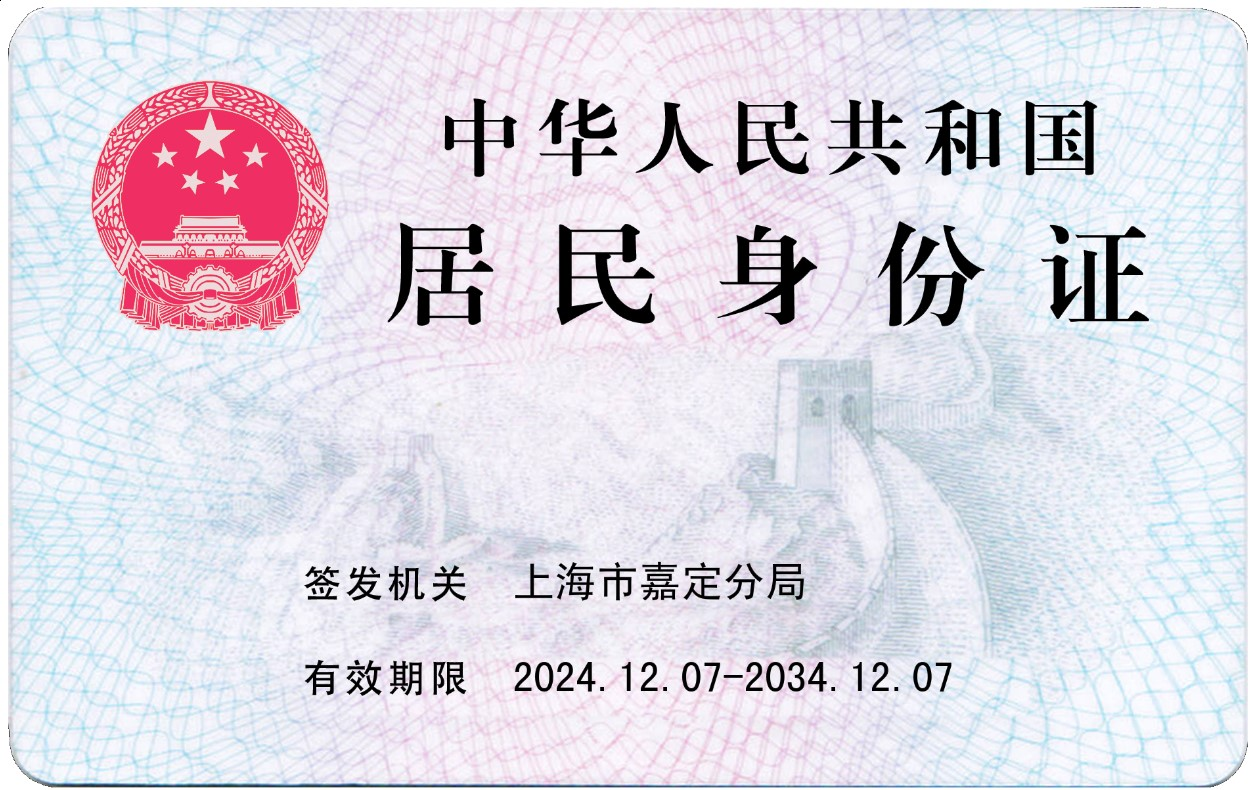
\includegraphics[width=\textwidth]{image/back.jpg} 
	\end{minipage}%
	\hfill
	\begin{minipage}[t]{0.51\textwidth}
		\begin{textblock*}{2cm}(11cm,11cm) % 可以自行增加国徽图标:设置图片的位置,(x, y) 为起始坐标
			%\includegraphics[width=2cm]{image/emblem.jpg} 
		\end{textblock*}
		\begin{tcolorbox}[colframe=black, colback=white]
			\begin{spacing}{1.3}
				\centering
				
				\vskip 0.4cm
				
				\textbf{The People's Republic of China}\\
				{\large \textbf{Resident Identification Card}}\\
				
				\vskip 0.8cm
				
				{\scriptsize \textbf{Issuing Authority:} Shanghai Public Security Bureau}\\
				{\scriptsize \textbf{Valid Period:} Dec 7,2024 - Dec 7,2034}
			\end{spacing}
		\end{tcolorbox}
	\end{minipage}
	
	\vspace{1cm}
	\begin{flushleft}
		\textbf{Notes:}
		\begin{itemize}
			\item Images on the left represent the front and back of the original Chinese ID card.
			\item The translations on the right correspond to the text fields of the ID card.
		\end{itemize}
	\end{flushleft}
\end{document}